\section{Entwurf} \thispagestyle{nomarkstyle}

\subsection{Datenmodell}
Beim Etnwurf des Datenmodells wurde darauf geachtet, es möglichst schlank zu halten und nur benötigte Informationen zu speichern.
Die grundlegenden Entitäten sind:
\begin{itemize}
\item\textbf{User.} Die registrierten Benutzer
\item\textbf{Address.} Adressdaten der Benutzer
\item\textbf{BaseItem.} Artikeldaten
\item\textbf{Category.} Kategorien
\item\textbf{ShoppingCart.} Warenkorb
\item\textbf{ShoppingOrder.} getätigte Bestellungen

Abbildung \ref{fig:ERM} zeigt das Datenmodell in der Gesamtsicht.
\begin{figure}[th!]
	\centering
	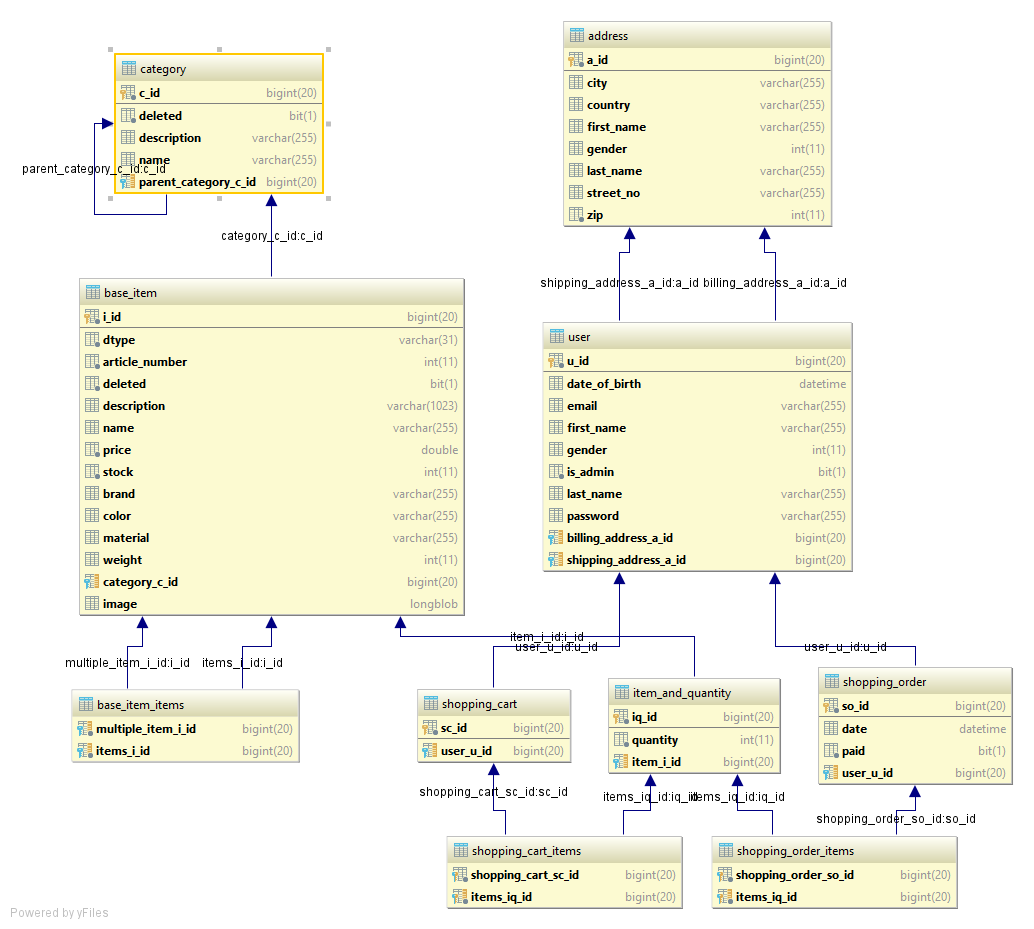
\includegraphics[width=\linewidth]{bilder/kap6/erm_diagram.png}
	\caption{Entity Relationship Modell}
	\label{fig:ERM}
\end{figure}

Die Beziehungen zwischen den Entitäten sind entweder direkt per Fremdschlüssel oder über Beziehungstabellen dargestellt und werden im Folgenden kurz beschrieben.
Ein User hat eine Lieferadresse (Shipping address) und eine Rechnungsadresse (Billing address).
Um die bereits angesprochene Hierarchie von Kategorien abzubilden, können Kategorien eine Eltern-Kategorie haben (Parent category).
Jeder Artikel ist genau einer Kategorie zugeordnet. Für die im Shop so genannten Sets mit mehreren Artikeln, gibt es eine zusätzliche Tabelle, die einem Set mehrere Einzel-Artikel zuordnen kann.
Die Warenkörbe sind immer einem Benutzer zugeordnet. In gleicher Weise sind auch die Bestellungen Benutzer-spezifisch.
Um der Tatsache gerecht zu werden, dass in einem Warenkorb oder in einer Bestellung Artikel mehrmals vorhanden sein können (wenn ein Benutzer von einem Artikel mehrere Exemplare bestellt), wurde eine zusätzliche Entität eingeführt.
Diese ItemAndQuantity genannte Entität hält jeweils eine Referenz auf einen Artikel, sowie eine Anzahl für diesen Artikel.
Warenkörbe und Bestellungen enthalten also immer Einträge aus dieser Tabelle.
Auf diese Weise genügt es, für einen Artikel immer nur einen Eintrag zu haben, auch wenn die bestellte Menge größer ist.
Ohne diese Lösung müsste es für eine Bestellung von beispielsweise dreißig Exemplaren eines Artikels auch dreißig Einträge geben.

\subsection{Schnittstellen}
%TODO Klassendiagramme

\subsection{Design der Weboberfläche}
%TODO UI Mockups